% ---- SECTION CONTEXTE ET ÉTAT DE L'ART ----

% -------------------------------------------------------
\section{La filière soja au Bénin (\textit{Glycine max})}
% -------------------------------------------------------

\subsection{Importance agronomique et économique}
Le soja (\textit{Glycine max}) est une légumineuse annuelle de la famille des \textit{Fabaceae}, originaire d'Asie de l'Est \cite{ifdcsoy}. Sa double valeur — nutritionnelle (environ 40~\% de protéines et 20~\% de lipides par masse sèche) et agronomique (fixation de l'azote atmosphérique par symbiose avec \textit{Bradyrhizobium japonicum}) — en fait une culture stratégique mondiale.

\begin{figure}[H]
    \centering
    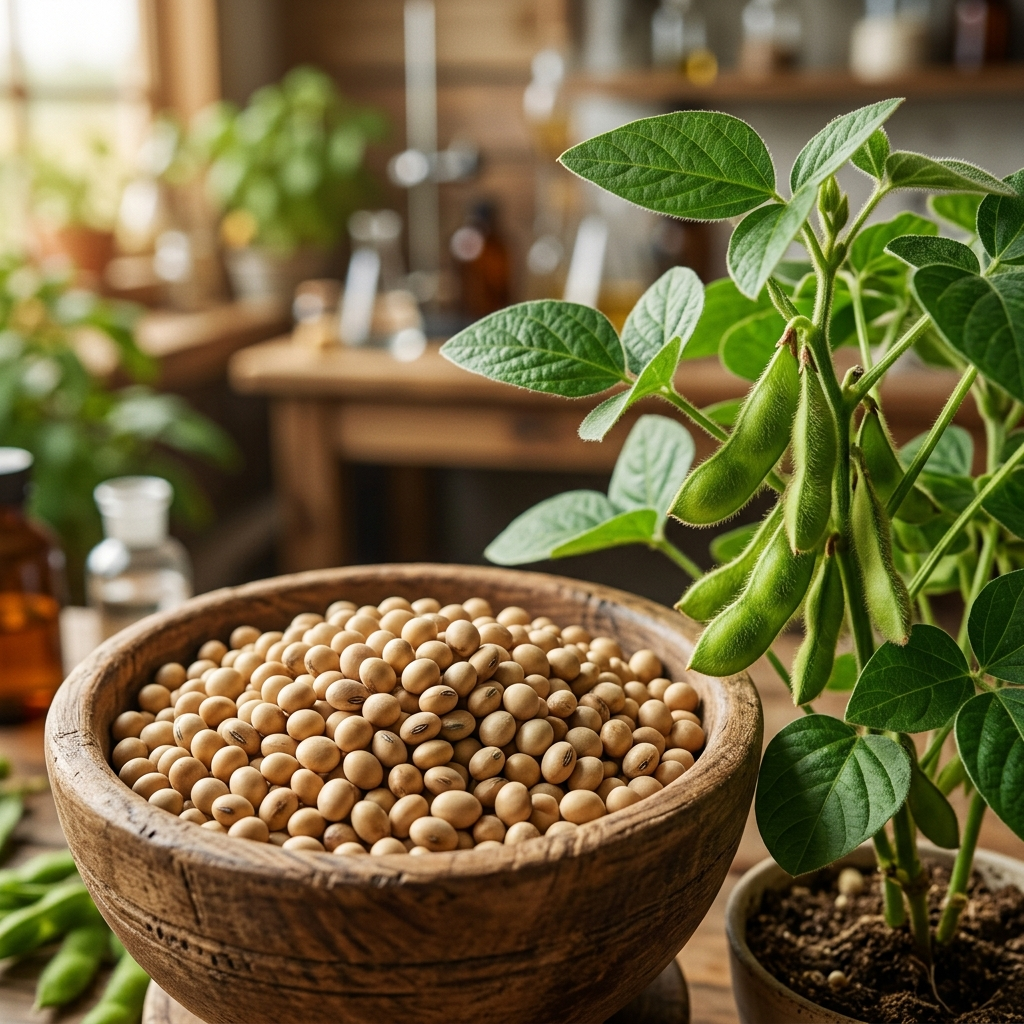
\includegraphics[width=0.45\textwidth]{images/soybean_premium.png}
    \caption{Plante de soja et ses graines (\textit{Glycine max})}
    \label{fig:soybean}
\end{figure}

Au Bénin, la production nationale a connu une progression fulgurante, passant de 157\,620 tonnes en 2015 à plus de 257\,000 tonnes en 2020 \cite{tidjani2023, faostat}, faisant du soja la 4\ieme{} source de devises du pays. Le soja est transformé localement en produits alimentaires (\textit{Wara}, lait, farines infantiles), jouant un rôle vital dans la lutte contre la malnutrition \cite{brab187}. Les variétés les plus répandues appartiennent à la série \textbf{TGX} (TGX 1448-2E, TGX 1910-14F, TGX 1835-10E), sélectionnées pour leur rendement et leur résistance.

\subsection{Enjeux qualitatifs et normes industrielles}
L'émergence de la Zone Industrielle de Glo-Djigbé (GDIZ) constitue le moteur d'une transformation structurelle de la filière \cite{gdiz2023}. Ces unités de trituration modernes imposent des standards stricts, encadrés par l'Agence Nationale de Normalisation à travers la norme \textbf{NB 01.07.004} \cite{anm_soja}. Cette norme, homologuée en 2021, vise à harmoniser les standards de qualité du soja béninois avec les exigences du marché international et des unités de transformations locales :

\begin{enumerate}
    \item \textbf{Taux d'humidité $<$ 12~\% :} Seuil critique pour prévenir les moisissures et assurer la performance des presses à huile.
    \item \textbf{Pureté spécifique $>$ 98~\% :} Absence de débris végétaux, cailloux ou grains brisés.
    \item \textbf{Intégrité du grain :} Limitation des grains cassés pour ne pas altérer la qualité du tourteau.
\end{enumerate}

Or, le diagnostic réalisé par le MAEP et l'UNPS révèle une rupture critique \cite{maep2023, unps2014} : le battage traditionnel et le séchage au sol ne permettent pas d'atteindre ces standards, entraînant des pertes post-récolte de 15~\% à 25~\% et un refoulement régulier des camions aux portes des usines.

\subsection{Étude de l'existant et limites des solutions actuelles}
Plusieurs approches coexistent, mais aucune ne répond simultanément aux contraintes rurales de mobilité, d'autonomie et de traçabilité :

\begin{table}[H]
    \caption{Analyse comparative des solutions de pré-traitement du soja}
    \label{tab:comparaison_soja}
    \centering
    \small
    \renewcommand{\arraystretch}{1.6}
    \rowcolors{2}{white}{lightGray}
    \begin{tabularx}{\textwidth}{|L|C|C|C|}
        \hline
        \rowcolor{lightGray}
        \textbf{Critères} &
        \textbf{Tri Manuel} &
        \textbf{Unités Importées} &
        \textbf{SMART-SOJA} \\ \hline
        Mobilité & Totale & Moyenne & \textbf{Optimisée} \\ \hline
        Source d'énergie & Humaine & Diesel / Réseau & \textbf{Solaire (Autonome)} \\ \hline
        Contrôle humidité & Aléatoire & Non mesurée & \textbf{Précis (Capteur)} \\ \hline
        Traçabilité Internet des objets & Aucune & Aucune & \textbf{Enregistrement numérique au format JSON} \\ \hline
        Accessibilité financière & Nul & Élevé & \textbf{Abordable / Modulaire} \\ \hline
    \end{tabularx}
\end{table}

La solution \textbf{SMART-SOJA} se positionne ainsi comme une approche innovante adaptée au contexte rural : elle déplace la technologie vers la ressource, en garantissant la conformité du grain avant tout acheminement industriel. 

Comme l'illustre le Tableau~\ref{tab:comparaison_soja}, la solution SMART-SOJA surpasse les alternatives existantes sur plusieurs dimensions clés. Contrairement au tri manuel qui reste extrêmement fastidieux, lent et incapable de quantifier scientifiquement le taux d'humidité, notre prototype intègre une mesure électronique précise et reproductible par double sonde capacitive. Par ailleurs, par rapport aux unités de traitement industrielles importées qui exigent un raccordement au réseau triphasé ou l'usage de générateurs diesel polluants et coûteux, SMART-SOJA garantit une autonomie énergétique totale en zone rurale grâce à son alimentation photovoltaïque 12~V. Enfin, sa capacité unique de traçabilité numérique et de communication IoT (génération de payloads JSON via le protocole MQTT) sécurise la chaîne d'approvisionnement en fournissant aux usines de la GDIZ un historique de qualité infalsifiable pour chaque lot avant son transport, réduisant à néant le risque de refoulement aux portes des usines.

% -------------------------------------------------------
\section{Technologies de tri et de nettoyage des grains}
% -------------------------------------------------------

\subsection{Principes physiques de séparation}
La littérature distingue trois principes fondamentaux pour séparer les grains de leurs impuretés \cite{fellows2009, brennan2006} :

\begin{figure}[H]
    \centering
    \begin{subfigure}[b]{0.32\textwidth}
        \centering
        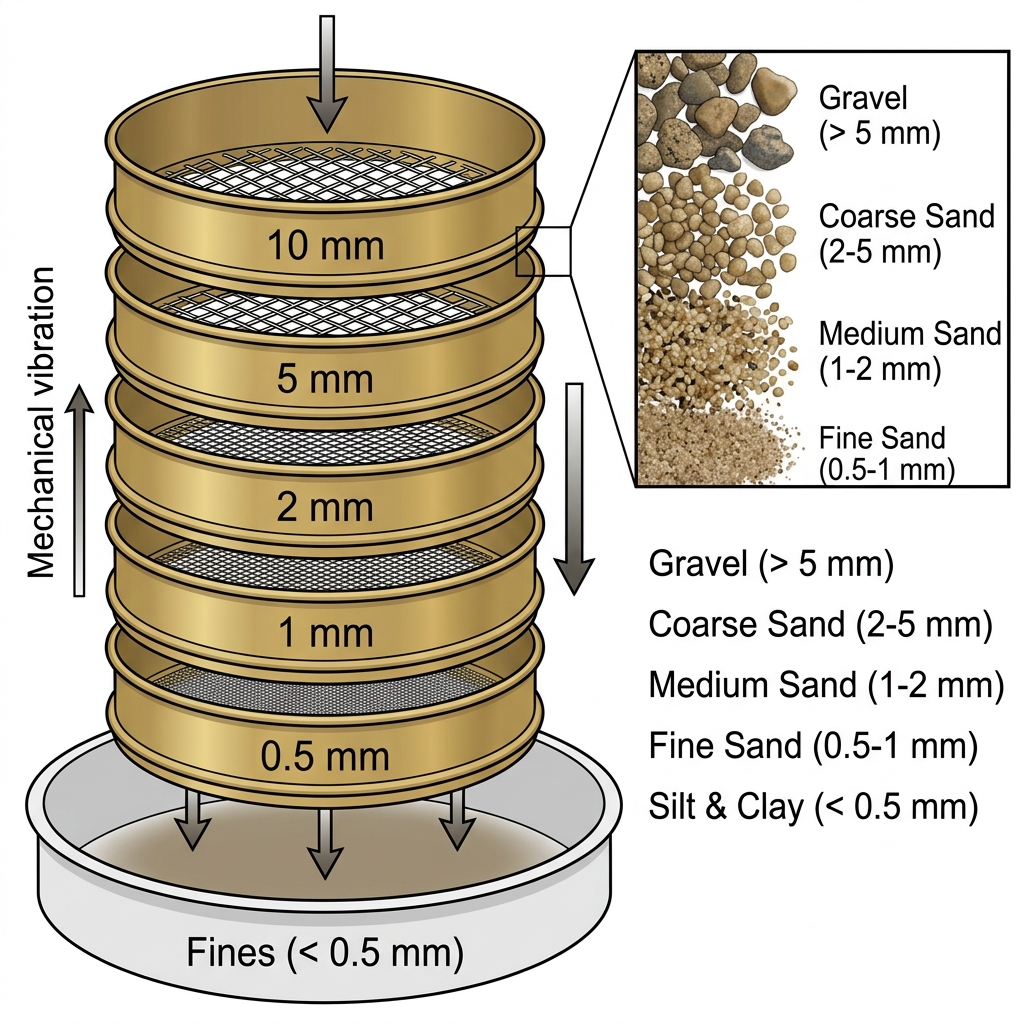
\includegraphics[width=\textwidth]{images/granulometrie.png}
        \caption{Séparation granulométrique}
    \end{subfigure}
    \hfill
    \begin{subfigure}[b]{0.32\textwidth}
        \centering
        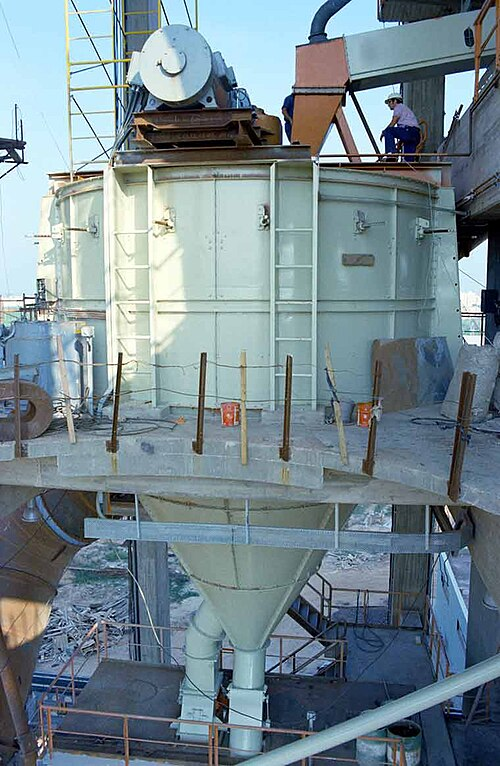
\includegraphics[width=\textwidth, height=4.5cm, keepaspectratio]{images/Zoubov-Sturtevant-whirlwind-centrifugal-Air-classifier-air-separator.jpg}
        \caption{Séparation aéraulique}
    \end{subfigure}
    \hfill
    \begin{subfigure}[b]{0.32\textwidth}
        \centering
        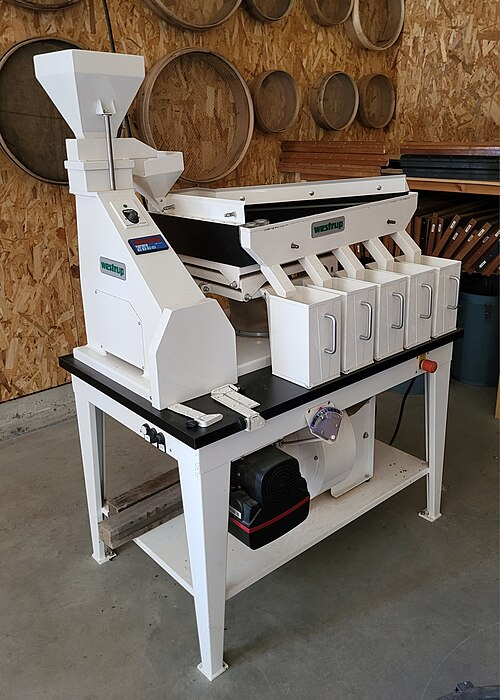
\includegraphics[width=\textwidth, height=4.5cm, keepaspectratio]{images/Table_densimétrique12.jpg}
        \caption{Séparation densimétrique}
    \end{subfigure}
    \caption{Principes physiques de triage des grains}
    \label{fig:tri_physique}
\end{figure}

\begin{itemize}
    \item \textbf{Séparation granulométrique :} Tamis vibrants ou rotatifs classant les grains selon leur taille et leur épaisseur (principe retenu pour le Bloc 2 de SMART-SOJA).
    \item \textbf{Séparation aéraulique :} Flux d'air vertical emportant les impuretés légères (poussières, gousses vides) tout en conservant les grains lourds.
    \item \textbf{Séparation densimétrique :} Table densimétrique exploitant un lit fluidisé pour trier des éléments de même taille mais de densités différentes.
\end{itemize}

\subsection{État de l'art industriel}
Au niveau industriel, les trieurs optiques représentent la solution la plus avancée : ils utilisent des caméras haute résolution et des algorithmes de traitement d'image pour éjecter les grains défectueux par jets d'air comprimé \cite{mahajan2015}. Bien que performants, leur coût élevé et leurs besoins énergétiques importants les rendent inaccessibles aux petits producteurs ruraux, justifiant une approche mécatronique plus abordable pour SMART-SOJA.

\begin{figure}[H]
    \centering
    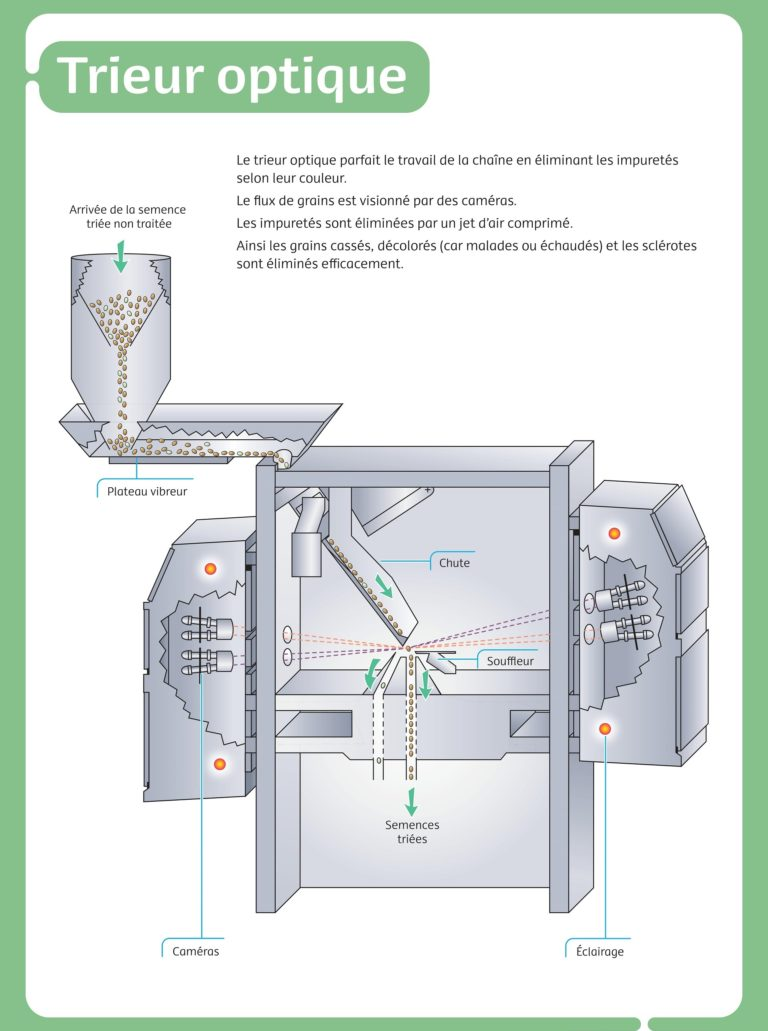
\includegraphics[height=6cm, keepaspectratio]{images/semae-pedagogie-station-semences-trieur-optique-768x1031.jpg}
    \caption{Exemple de trieur optique industriel haute résolution (Source : SEMAE Pédagogie)}
    \label{fig:trieur_optique}
\end{figure}

\FloatBarrier

% -------------------------------------------------------
\section{L'Internet des objets dans le secteur agricole (Agriculture 4.0)}
% -------------------------------------------------------

\subsection{Réseaux de capteurs sans fil (WSN) et connectivité LPWAN}
L'intégration de l'Internet des objets en agriculture (\textit{Smart Farming}) transforme la collecte et l'exploitation des données de terrain \cite{tarekegn2020}. Pour les zones rurales, les technologies \textbf{LPWAN} (\textit{Low-Power Wide-Area Network}) sont particulièrement adaptées en raison de leur longue portée et de leur faible consommation énergétique \cite{hanes2017, tzounis2017}.

\begin{figure}[H]
    \centering
    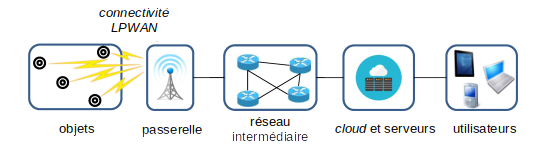
\includegraphics[width=0.65\textwidth]{images/Sensors-LPWAN.png}
    \caption{Architecture de connectivité LPWAN pour capteurs agricoles}
    \label{fig:iot_connectivity}
\end{figure}

Le protocole \textbf{MQTT} (\textit{Message Queuing Telemetry Transport}) constitue le standard de facto de l'Internet des objets industriel léger : son architecture Publication/Abonnement permet une communication robuste sur des réseaux à bande passante limitée et connexion instable, comme les zones rurales du Bénin \cite{mqtt_org, hanes2017}.

\subsection{Traçabilité numérique et Big Data agricole}
La numérisation des données de qualité crée un \textit{passeport numérique} du grain depuis le champ jusqu'à l'usine. Les travaux de recherche montrent que la structuration de ces données en format \textbf{JSON} permet de limiter les fraudes, de garantir les standards qualité de la GDIZ et d'ouvrir la voie à des analyses prédictives (Big Data agricole) pour l'amélioration continue des processus.


\subsection{Autonomie énergétique en milieu rural}
L'électrification rurale étant défaillante dans de nombreuses zones de production, la littérature technique privilégie les systèmes photovoltaïques hybrides avec régulateurs \textbf{MPPT} (\textit{Maximum Power Point Tracking}) pour optimiser l'extraction d'énergie solaire, abondante dans les régions tropicales comme le Bénin.

\FloatBarrier

% -------------------------------------------------------
\section{Cahier des charges fonctionnel}
% -------------------------------------------------------

L'analyse du contexte de la filière soja, des exigences normatives (NB~01.07.004) et des limites des solutions existantes permet de formuler le cahier des charges fonctionnel du système SMART-SOJA. Ce document de référence définit les fonctions que le prototype doit remplir, les critères d'acceptation et les moyens de validation associés. Les fonctions sont classées en \textbf{fonctions principales} (FP), directement liées aux objectifs du système, et en \textbf{fonctions contraintes} (FC), imposées par l'environnement d'utilisation.

\subsection{Fonctions principales}

Le Tableau~\ref{tab:cdc_fp} détaille les sept fonctions principales du système, issues des objectifs spécifiques du mémoire et des exigences de la norme \textbf{NB~01.07.004}.

\begin{table}[H]
    \caption{Cahier des charges fonctionnel — Fonctions principales (FP)}
    \label{tab:cdc_fp}
    \centering
\footnotesize
\renewcommand{\arraystretch}{1.5}
\rowcolors{2}{white}{lightGray}
\begin{tabularx}{\textwidth}{|p{2.3cm}|L|p{2.1cm}|L|L|}
\hline
\rowcolor{lightGray}
\textbf{Fonction} & \textbf{Exigence} & \textbf{Valeur cible} & \textbf{Justification} & \textbf{Moyen de vérification} \\ \hline

\textbf{FP1}\newline Nettoyage &
Séparer les impuretés des grains par tamisage vibrant &
Pureté $>$ 98~\% &
Norme NB~01.07.004, exigence GDIZ &
Pesée différentielle avant/après, inspection visuelle \\ \hline

\textbf{FP2}\newline Mesure humidité &
Mesurer le taux d'humidité en deux points du lot (Soil1/Soil2) &
$\pm\,5$~\% HR, seuil 12~\% &
Norme NB~01.07.004 &
Comparaison avec hygromètre de référence certifié \\ \hline

\textbf{FP3}\newline Séchage actif &
Réduire l'humidité par air chaud et brassage si $H > 12$~\% &
$H \leq 12$~\% en sortie (double validation) &
Prévention moisissures, conformité GDIZ &
Lecture convergente Soil1 ET Soil2 $\leq$ 12~\% \\ \hline

\textbf{FP4}\newline Pesée &
Peser chaque lot traité avec précision &
0--10~kg, $\pm\,0{,}1$~\% &
Certification du poids pour traçabilité &
Étalonnage poids de référence (module HX711) \\ \hline

\textbf{FP5}\newline Traçabilité IoT &
Générer un passeport numérique JSON par lot et le transmettre via MQTT &
Payload JSON complet, publication MQTT &
Transparence et fiabilité de la chaîne d'approvisionnement &
Réception et décodage sur broker HiveMQ \\ \hline

\textbf{FP6}\newline Autonomie &
Fonctionner en autonomie solaire hors réseau électrique &
$\geq$ 3~h/jour, recharge solaire en 5~h &
Zones rurales non électrifiées &
Mesure tension batterie, durée de cycle effective \\ \hline

\textbf{FP7}\newline Mobilité &
Déplacer l'unité vers les sites de collecte &
Châssis sur roulettes, compatible véhicule utilitaire &
Rapprocher la technologie du producteur &
Test de déplacement sur terrain plat et piste \\ \hline

\end{tabularx}
\end{table}

\subsection{Fonctions contraintes}

Le Tableau~\ref{tab:cdc_fc} regroupe les contraintes imposées par l'environnement opérationnel, la sécurité et la maintenabilité du système.

\begin{table}[H]
    \caption{Cahier des charges fonctionnel — Fonctions contraintes (FC)}
    \label{tab:cdc_fc}
    \centering
\footnotesize
\renewcommand{\arraystretch}{1.5}
\rowcolors{2}{white}{lightGray}
\begin{tabularx}{\textwidth}{|p{2.3cm}|L|p{2.1cm}|L|L|}
\hline
\rowcolor{lightGray}
\textbf{Fonction} & \textbf{Exigence} & \textbf{Valeur cible} & \textbf{Justification} & \textbf{Moyen de vérification} \\ \hline

\textbf{FC1}\newline Interface opérateur &
Affichage et contrôle local du cycle &
LCD 16$\times$2, 2 potentiomètres, boutons, LEDs &
Opérateur non expert en milieu rural &
Test d'utilisabilité en conditions réelles \\ \hline

\textbf{FC2}\newline Contrôle temps réel &
Automatisation séquentielle (GRAFCET) avec sécurité prioritaire &
Temps de réponse sécurité $<$ 10~ms &
Sûreté de fonctionnement, arrêt d'urgence &
Test arrêt d'urgence, chronogramme FreeRTOS \\ \hline

\textbf{FC3}\newline Résilience réseau &
Aucune perte de données en l'absence de WiFi &
\textit{Store-and-Forward} sur carte MicroSD &
Couverture WiFi limitée en zone rurale &
Test déconnexion/reconnexion, intégrité données \\ \hline

\textbf{FC4}\newline Maintenabilité &
Accès individuel aux sous-systèmes sans démontage intégral &
4 blocs amovibles, connecteurs rapides &
Maintenance en milieu rural isolé &
Démontage et remontage d'un bloc $<$ 15~min \\ \hline

\textbf{FC5}\newline Robustesse &
Résistance aux vibrations, poussière et chocs de transport &
Châssis acier 40~mm, tamis inox 304, roulettes caoutchouc &
Usage en extérieur, transport sur pistes &
Inspection visuelle après campagne de tests \\ \hline

\textbf{FC6}\newline Coût &
Accessibilité financière du prototype &
Composants standard, disponibles localement &
Cible : coopératives et petits producteurs &
Bilan financier détaillé des composants \\ \hline

\end{tabularx}
\end{table}

Ce cahier des charges constitue le document de référence pour la suite de l'étude. Chaque fonction sera traitée dans les sections suivantes à travers les choix d'architecture, de composants et de dimensionnement du système SMART-SOJA.

% Fin de la section contexte
